% Attempting to convert solutions to docx and then go from there.

\documentclass[lang=en]{skrapport}
\nonstopmode
\usepackage[utf8]{inputenc}
\usepackage{graphicx}
\usepackage{amsmath,amssymb}
\usepackage[ocgcolorlinks]{hyperref}
\usepackage{tabularx}
\usepackage{booktabs}
%\usepackage[american,siunitx]{circuitikz}
%\newcommand{\equal}{=}
\usepackage{float}
\usepackage{siunitx}
\usepackage{enumitem}
\usepackage{tikz}
\usepackage{bodegraph}
\begin{document}
\begin{quote}
\emph{\textbf{ELEC 300 --- Linear Circuits: II --- Spring 2018}}
\emph{\textbf{Name \_\_\_\_\_\_\_\_\_\_\_\_\_\_\_\_\_\_\_}}
\end{quote}


\includegraphics[width=0.47222in,height=0.59236in]{media/image1.jpeg}

\begin{quote}
\emph{\textbf{Assignment 04 --- due Monday, 05 Feb 2018, in class}}
\emph{\textbf{Std \#\_\_\_\_\_\_\_\_\_\_\_\_\_\_\_\_\_\_\_\_}}
\end{quote}

\textbf{\emph{Problem 1}}

A coil with a resistance of 5 and inductance 100 mH is connected in
series with a capacitor of 50 pF. The circuit is connected to a voltage
source that provides 1 V at all frequencies and has an

inner impedance of 50 . Calculate \emph{o}, \emph{Q} and \emph{B}.

\textbf{\emph{Problem 2}}

The parameters of a parallel \emph{RLC} circuit are \emph{R} = 100 k ,
\emph{L} and \emph{C} = 40 pF. The circuit is

driven by a current source with an inner impedance of 1 M . Calculate
the quality factor, the center frequency, and the half power
frequencies.


%% Chapter 14-36 Alexander 
\textbf{\emph{Problem 3}}

Design a parallel \emph{RLC} circuit that has a midband admittance of 25
10\textsuperscript{-3} S, quality factor of 80, and a resonant frequency
of 200 krad/s. Calculate the values of \emph{R}, \emph{L}, and \emph{C}.

\textbf{\emph{Problem 4}}

Find the resonant frequency.

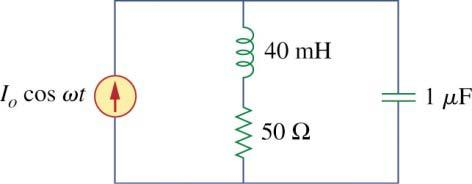
\includegraphics[width=2.14167in,height=0.83611in]{media/image2.jpeg}

\textbf{\emph{Problem 5}}

Find the transfer functions \emph{H}( ) =\emph{IL}( )/\emph{Is}( ) and
determine the relationship between the damping factor and the quality
factor \emph{Q}.

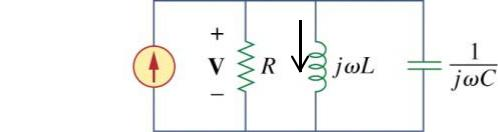
\includegraphics[width=2.99792in,height=0.79514in]{media/image3.jpeg}


\end{document}